
\section{Finding the solution}
In \corRef{liftDescr} we have seen that horizontal curves can be written as
$z_t = g(t) \cdot z_0$ where $g$ is some curve in $\MSd$. Now we want to \emph{find}
such a $g$ so that $f(g(t) \cdot z_0) = \gamma(t)$ for all $t$ where
$\gamma : [0,1] \rightarrow \Rd$. That is the snout of $S_{z_t}$ follows $\gamma$.

Recall the definition of the \term{gradient}: let $\varphi : M \rightarrow \R$ be
a map. The gradient $\grad \varphi$ is a function
$M \rightarrow TM$ \st $\grad \varphi(x)$ points in the direction of the greatest
rate of increase of $\varphi$ at $x$. Formally this needs $M$ to be a Riemannian
manifold (a manifold with a differentiable inner product on the
tangent space), but this short description should suffice for the understanding
of the rest. For more details see \cite[p. 38 + 83]{Carmo} or \cite[p. 123]{Kaballo97}.

Now consider the family of maps
    \[ \xi_v = \grad (\varphi_v \circ f) : \Conf \rightarrow T \Conf \]
where $\varphi_v(x) = \inner{x}{v}$. The meaning of this is the following: take
a vector $v$ and a configuration $z$ then $\xi_v(z) \in T_z\Conf$ is a change of $z$
\st the snout follows $v$.

Now let us take this a step further by the map
    \[ v \mapsto T_zf(\xi_v(z)) . \]
This map gives now the direction in which the snout moves if we deform $z$ \st the
snout follows $v$ maximally. It is easy to prove that for fixed $z$ this map is linear
and so gives rise to a matrix $M(z)$. The exact definitions and calculation are given
in \cite{Rodriguez07}.

\subsection{Another property of the solution}

We will use $M^{-1}(z)$ to describe the solution so we need to know when $M(z)$
is invertible. By definition of $T_z\Conf$ and $M(z)$ this equivalent to finding the
critical points of $f$, that is elements of $\ker T_zf$.

For this we inspect a special type of configurations.

\begin{definition}
    A configuration $z \in$ is said to be \term{lined} if there exists $p \in \Sd{d-1}$
    \st $z([0,L]) \subseteq \{\pm p\}$.
\end{definition}

These are called lined because the snake $S_z$ only moves in one straight line.

We can now find

\begin{lemma}\label{lem:critPoint}
    A configuration $z \in \Conf$ is a critical point of $f$ if and only if,
    it is lined (\cite[Proposition 2.6]{Rodriguez07}).
\end{lemma}

So $M(z)$ is invertible iff $z$ is not lined.

\theoRef{AccDescr} has another interesting consequence:
\begin{corollary}
    If an initial configuration $z_0 \in \Conf$ has $z_0(s) = z_0(s')$
    for $s,s' \in [0,L]$ then $z_t(s) = z_t(s')$ for all $z_t \in \mathcal{A}(z_0)$
    (\cite[Proposition 3.10]{Rodriguez07}).
    
    So if $z_0$ takes a finite number of different values, then so do all $z_t$.
\end{corollary}

Which in turn gives us

\begin{lemma}
    If $z_0 \in \Conf$ takes at least 3 distinct values, then there is no lined
    configuration in $\mathcal{A}(z_0)$.
\end{lemma}

So the necessary condition for the existence of $M^{-1}(z)$ is that $z$ takes at
least 3 distinct values.

\subsection{Charming the snake}
Now we are an the position to let the snake move.

\begin{theorem}
    Let $z_0 \in \Conf$ be a configuration which takes at least 3 distinct values and
    $\gamma \in \diff{1}{\I}{\Rd}$ with $f(z_0) = \gamma(0)$ and
    $\gamma(\I) \subseteq f(\mathcal{A}(z_0))$.
    
    Then there exists a time dependent vector field $X_t(g) \in T_g\MSd$ \st if
    $g : \I \rightarrow \MSd$ satisfies the ordinary differential equation
        \[ \dot{g}(t) = X_t(g(t)), \qquad g(0) = id_{\MSd} \]
    then $\widetilde{\gamma}(t) = g(t) \cdot z_0$ is the unique horizontal lift of
    $\gamma$ starting at $z_0$.
    
    \begin{proof}
        Let us look at the map $F : \MSd \rightarrow \Rd$ with $F(g) = f(g \cdot z_0)$.
        This translates a Möbius transformation into the position of the snout if it is
        applied to $z_0$. So its tangent map
        $T_gF : T_g\MSd \rightarrow T_{F(g)}\Rd = \Rd$ tracks changes of the snout
        if the transformation is changed.
        
        By \cite[p. 38]{Rodriguez06} there is a distribution
        $\Delta_g^{\mathcal{H}} \subseteq \MSd$ for some $\mathcal{H} \subseteq \MSd$
        which satisfies
            \begin{center}
            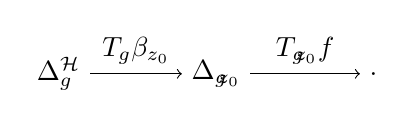
\begin{tikzpicture}[node distance=2cm, auto]
              \node (H) {$\Delta_g^{\mathcal{H}}$};
              \node (C) [right of=H] {$\Delta_{g \!\!\cdot\!\! z_0}$};
              \node (Rd) [right of=C] {$\Rd$.};
              \draw[->] (H) to node {$T_g\beta_{z_0}$} (C);
              \draw[->] (C) to node {$T_{g \!\!\cdot\!\! z_0}f$} (Rd);
            \end{tikzpicture}
            \end{center}
        Where $\beta_z(g) = g \cdot z \in \Conf$. This is a bijection.

        If we restrict this map to $T_gF|_{\Delta_g^{\mathcal{H}}}$
        this is equivalent to the Matrix $M(g \cdot z_0)$.
        Since $z_0$ takes at least 3 distinct values $M(g \cdot z_0)$
        is invertible for all $g \in \MSd$.
        
        The vector field $X_t(g)$ should give us a vector for every $g$ \st the snout
        follows $\gamma$:
            \[ M(g \cdot z_0) X_t(g) = \dot{\gamma}(t) . \]
        So $X_t(g) = M^{-1}(g \cdot z_0)\dot{\gamma}(t)$.
        
        Since $g(t)$ is the trajectory through $id$, we get that by construction
        $g(t) \cdot z_0$ is the unique horizontal lift of $\gamma$
        (see a text about initial value problems of ODEs).
    \end{proof}
\end{theorem}

\begin{remark}
    Note that there are cases where this differential equation does not have a solution
    for all $t$. This is discussed in \cite[Section 5]{Rodriguez07}.
\end{remark}

